\section{Introduction}

\begin{frame}[plain]
   \sectionpage
\end{frame}

\frame{
   \frametitle{Logistic management for healthcare systems}

   \textbf{Overview of HHCP}
   \begin{itemize}
      \item First study from \citeyear{fernandez1974}
      \item Home care: patients receive healthcare in their \emph{homes}
      \item Traditional systems: patients receive healthcare in \emph{hospitals}
   \end{itemize}

   \vspace*{12pt}

   \textbf{Ease the access to health and social care services}
   \begin{itemize}
      \item More inclusive
      \item Alternative to nursing homes
      \item Leverage hospital beds for complex cases
   \end{itemize}

   \vspace*{12pt}

   \textbf{Arriving challenge:} Efficient routing solution for caregivers to patient locations.


%   \todo[inline]{Add a example image with the flow of hospitals/patients/physicians}
}

\frame{
   \frametitle{Logistic management for healthcare systems}

   \textbf{Core of home care problems}: A vehicle routing problem with additional constraints.

   \vspace*{12pt}

   \only<+> {
      \begin{figure}[H]
         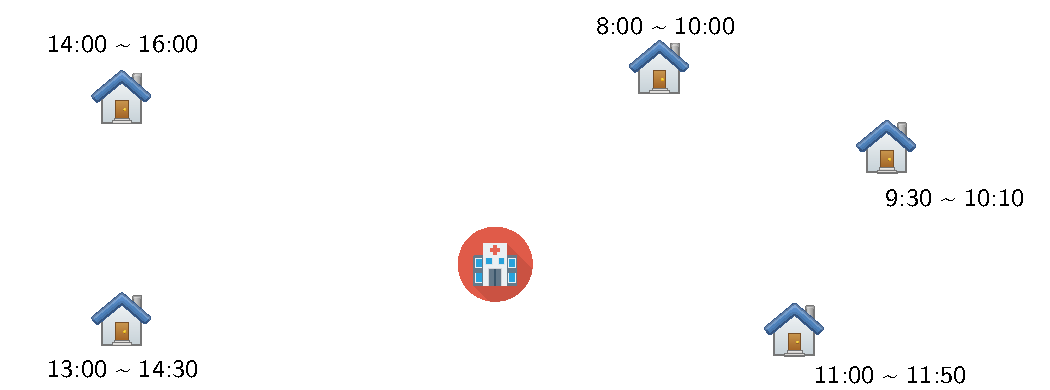
\includegraphics[width=0.8\textwidth, page=1]{fig/routing-example}%
      \end{figure}
   }

   \only<+> {
      \begin{figure}[H]
         \includegraphics[width=0.8\textwidth, page=2]{fig/routing-example}%
      \end{figure}
   }

   \only<+> {
      \begin{figure}[H]
         \includegraphics[width=0.8\textwidth, page=3]{fig/routing-example}%
      \end{figure}
   }

   \only<+> {
      \begin{figure}[H]
         \includegraphics[width=0.8\textwidth, page=4]{fig/routing-example}%
      \end{figure}
   }

   \only<+> {
      \begin{figure}[H]
         \includegraphics[width=0.8\textwidth, page=5]{fig/routing-example}%
      \end{figure}
   }

   \only<+> {
      \begin{figure}[H]
         \includegraphics[width=0.8\textwidth, page=6]{fig/routing-example}%
      \end{figure}
   }
}

%\frame{
%   \frametitle{Logistic management for healthcare systems}
%
%   \textbf{Arriving challenge:} Efficient routing solution for caregivers to patient locations.
%
%   \begin{itemize}
%      \item Reduces hospitalization costs
%      \item Decentralized care
%      \item Increases patients comfort
%      \item Reduces patient stress and the pressure of mental health
%   \end{itemize}
%}

\frame{
   \frametitle{Logistic management for healthcare systems}

   \textbf{Increased life expectancy}

   \only<1> {
   \begin{itemize}
      \item Population aging
      \item Exhaustion of public healthcare services
   \end{itemize}
   }

   \vspace*{8pt}

   \only<1,2> {
      \begin{figure}[H]

         \subfloat[Brazil in 2010]{
            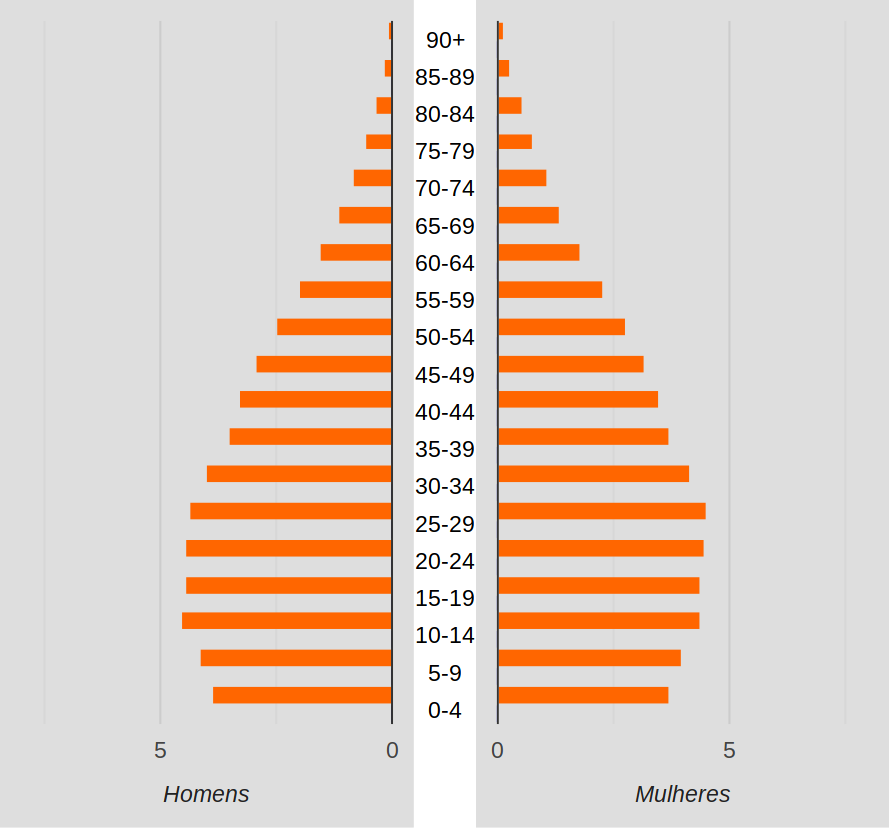
\includegraphics[width=0.29\textwidth]{fig/piramide-2010.png}

         }
         \hfill
         \subfloat[Brazil in 2021]{
           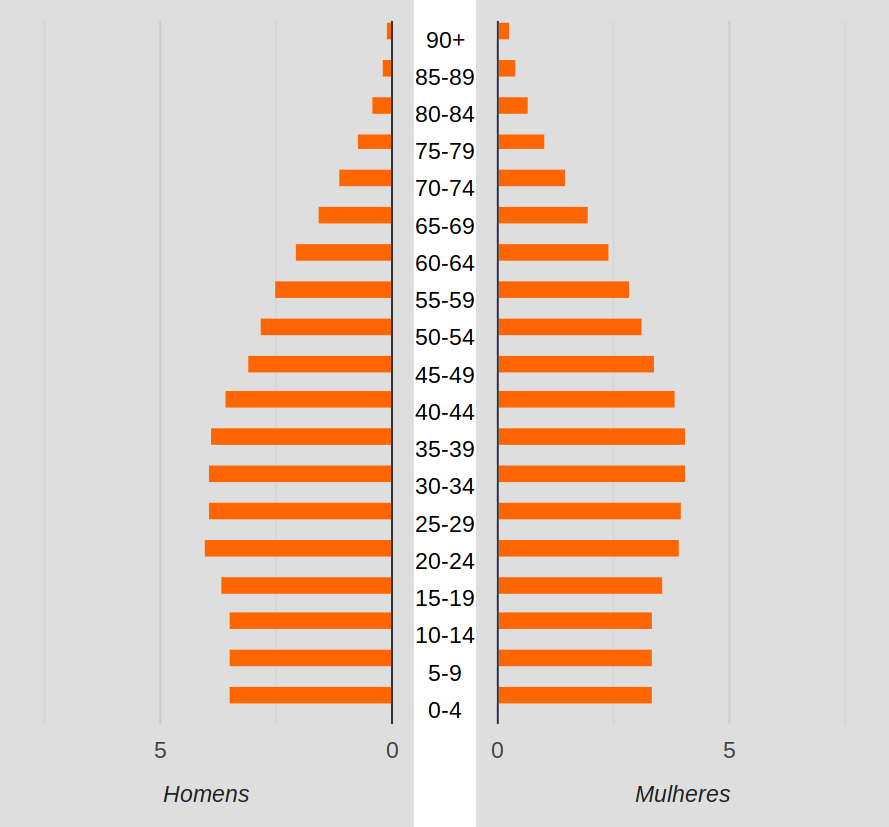
\includegraphics[width=0.29\textwidth]{fig/piramide-2021.png}

         }
         \hfill
         \subfloat[Brazil in 2050]{
            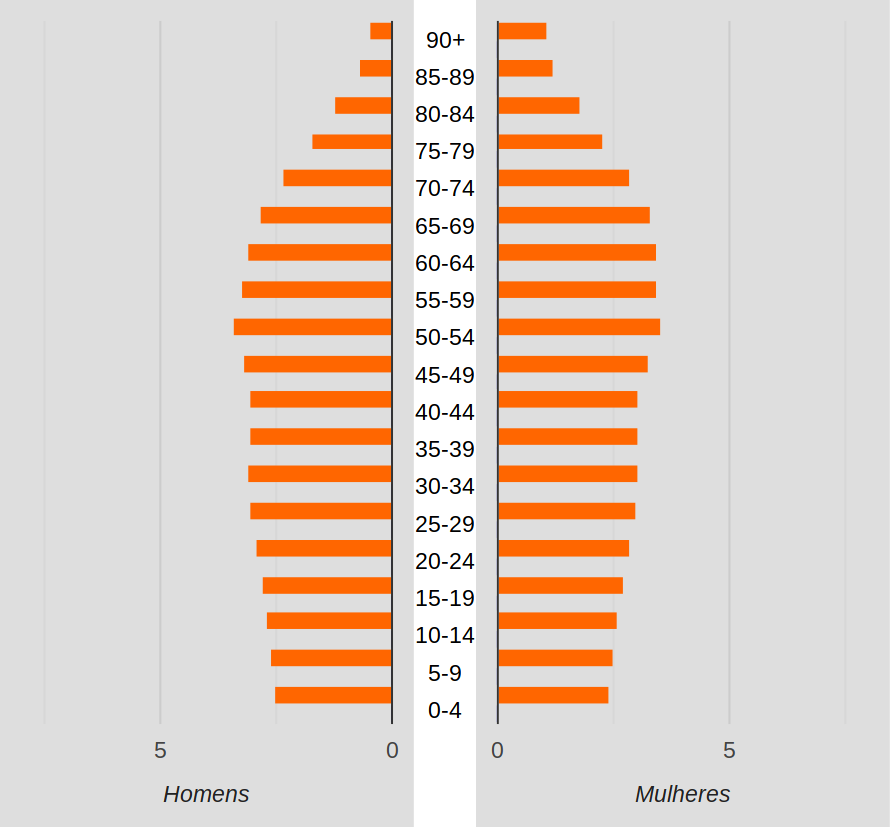
\includegraphics[width=0.29\textwidth]{fig/piramide-2050.png}

         }

         \caption{Source: Brazilian Institute of Geography and Statistics (2010)}

      \end{figure}
   }

   \only<2> {
%      \begin{figure}[H]
%         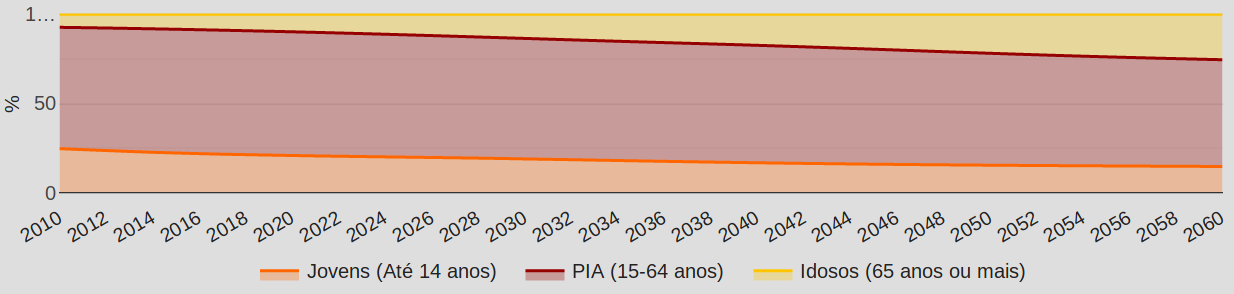
\includegraphics[width=\textwidth]{fig/brazilian-pop-evol.png}
%         \caption{Source: Brazilian Institute of Geography and Statistics (2010)}
%      \end{figure}

      Estimated population over 65+ years:
      \footnotesize
      \begin{itemize}
         \item In 2010: \phantom{0}7.32\% (14M people)
         \item In 2021: 10.15\% (21M people)
         \item In 2050: \color{InfRed} 21.87\% (51M people)
      \end{itemize}
   }
}

\frame{
   \frametitle{Logistic management for healthcare systems}

   \textbf{Healthcare services}
   \begin{itemize}
      \item Physiotherapy
      \item Dressing change
   \end{itemize}

   \vspace*{12pt}

   \textbf{Social care services}
   \begin{itemize}
      \item Preparation of meals
      \item Bathing, laundry
      \item House cleaning
   \end{itemize}
}



\frame{
   \frametitle{Logistic management for healthcare systems}

   \begin{tikzpicture}[overlay]
   \node at (9.5,-0.3) {
\includegraphics[scale=0.4]{fig/snapshot-covid}} ;
   \end{tikzpicture}

   \vspace{4pt}

   \textbf{Covid-19 pandemic in Brazil}
   \begin{figure}[H]
      \subfloat[Total cases (\textasciitilde 14M)]{
         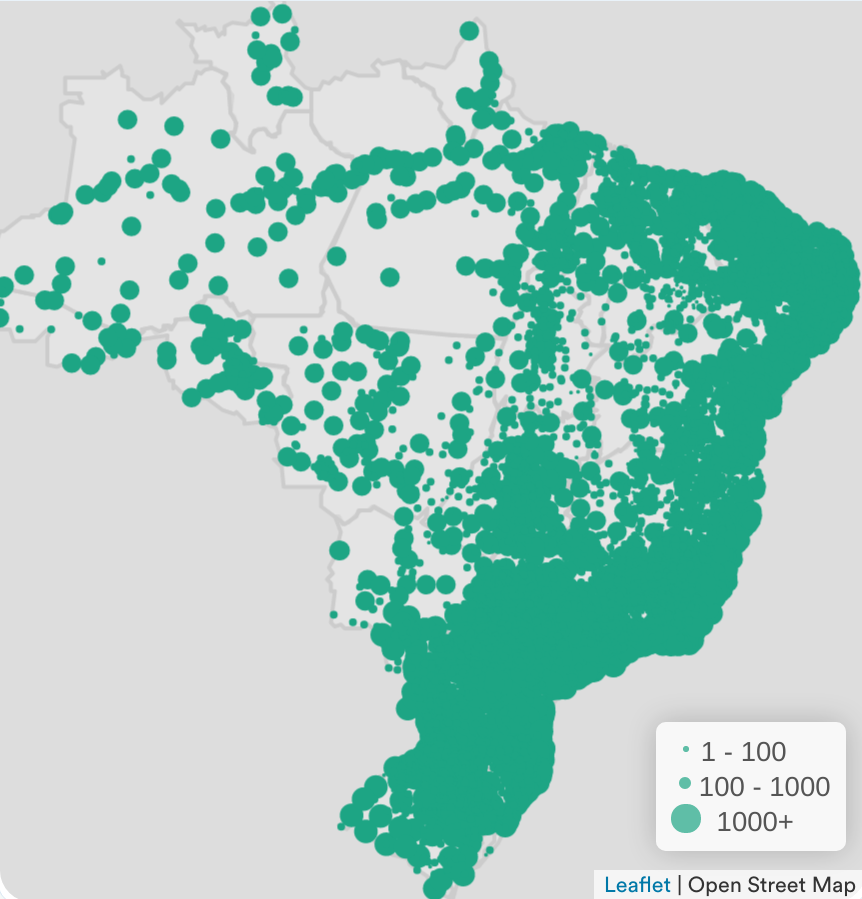
\includegraphics[width=0.4\textwidth]{fig/casos-covid}
      }
      \hfill
      \subfloat[Total deaths (\textasciitilde 378k)]{
         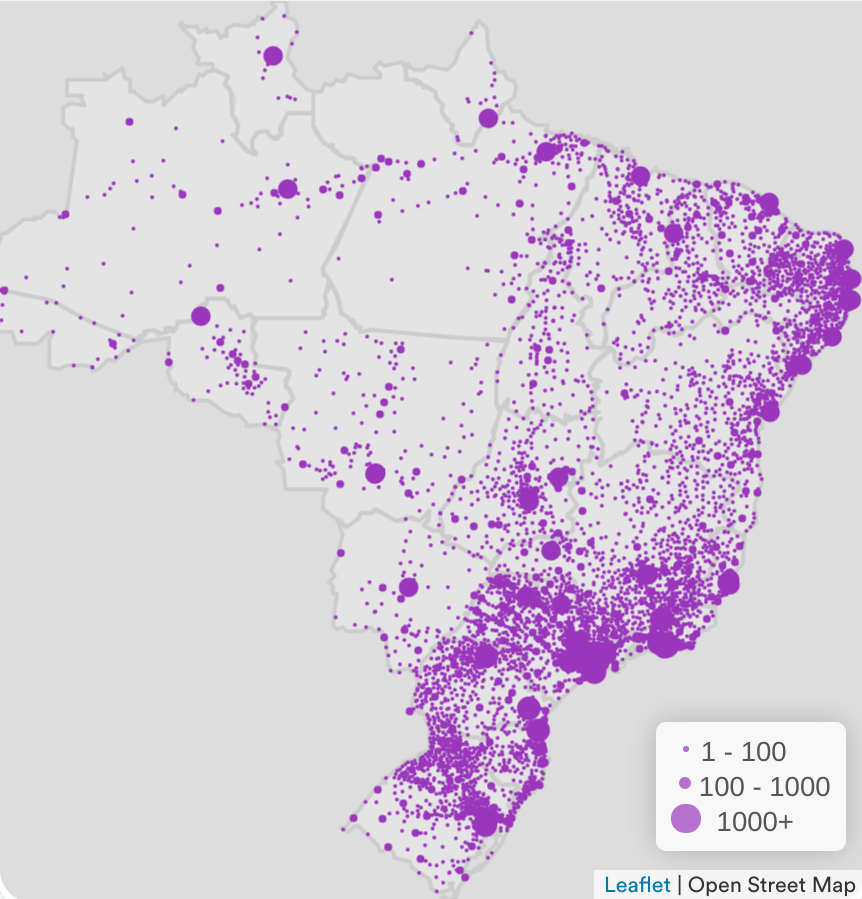
\includegraphics[width=0.4\textwidth]{fig/obitos-covid}
      }
      \caption{Source: DATASUS (2021)}
   \end{figure}
}

\frame{
   \frametitle{Logistic management for healthcare systems}

   \textbf{Covid-19 pandemic in Brazil}
   \begin{itemize}
      \item Lack of testing
      \item Lack of monitoring
   \end{itemize}

   \vspace{12pt}

   \textbf{But our public health system could be doing more}
   \begin{itemize}
      \item \emph{Better in Home}: pilot HHC program
%      \item Before the pandemic: weekly visit by health agents
      \item In Porto Alegre: vaccination through HHC structure
   \end{itemize}
}